\documentclass[12pt,a4paper]{article}
\setlength{\topmargin}{-5mm}
\setlength{\textheight}{244mm}
\setlength{\oddsidemargin}{0mm}
\setlength{\textwidth}{165mm}

\usepackage{fancyvrb}
\DefineVerbatimEnvironment{verbatim}{Verbatim}{xleftmargin=4mm}

\usepackage{lmodern}
\usepackage[T1]{fontenc}
\usepackage{pxfonts}
\usepackage{textcomp}
\usepackage{tabu}
\usepackage{graphicx}

\title{Luck and Roguelikes}
\author{Jeremy Mates}
\date{July 16, 2019}

\usepackage{hyperref}
\hypersetup{pdfauthor={Jeremy Mates},pdftitle={Luck and Roguelikes}}

\begin{document}
\maketitle

\setlength{\parindent}{0pt}

This began as a \texttt{README} file for pseudo random distribution
practice
code\footnote{\url{https://github.com/thrig/ministry-of-silly-vaults/tree/master/pseudo-random-dist}}
but at some point evolved into a longer discussion on randomness and
luck and related functions. \\

Some knowledge (but not much) of statistics and role playing games is
assumed. For the games aspect if you know what 3d6 means you will
probably be fine; for the statistics, a few Khan Academy videos or a
chapter or two of an introductory book on statistics should more than
suffice. You may also want to know a bit about C. And unix.

\section*{Pseudo Random Distributions}

Pseudo Random Distribution (PRD) are used in games to make the Random
Number Generator (RNG) less likely to go on long runs of hits or misses.
A RNG with more fibre in its diet, in other words. Briefly, when an
ability activates the chance of activation is reset to a very low value;
this value increases with each miss and will either reach 100\% or wrap
around to the lowest activation value depending on how the PRD is
designed (or it could segfault, but those versions tend to be fixed
before public release). The table of odds is usually designed such that
on average the chance of activation works out to some published
value\textendash say, 25\%\textendash though a PRD will have different
statistical properties than a straight check against the RNG. More on
this, later. \\

Use of a PRD reduces the influence of luck; without a PRD a mage may
fail their 75\% chance-to-activate spell three times in a row, die, and
then complain that the spell ``ought to'' activate somewhere around
three times out of four attempts, or otherwise certainly not fail three
times in a row, I mean did Gandalf ever flub a spell? No!
(etc.) This is the Gambler's Fallacy; a PRD attempts to make
the fallacy true. With a PRD the inverse will also be true; the mage
will be less likely to see multiple activations of their spell in a row
as the chance to activate decreases following each activation. \\

A downside of PRD is that state must be maintained. There may thus be
scaling issues as the number of abilities and entities tracked increase;
normal attacks might instead use the RNG directly to avoid this
problem\textendash possibly with multiple dice; 3d6 averages out better than a
similar roll of a 1d20\textendash and a PRD might only be used for select
abilities, possibly those that have tactical uses, or where too frequent
an activation would be as problematic as too rare, and the cost of
maintaining state is a necessary evil.

\section*{Enough with the Prose; Code}

\begin{verbatim}
#include <stdint.h>
#include <stdio.h>
#include <stdlib.h>

#define TRIALS 10000

#define PRD_COLS 7
uint32_t odds[PRD_COLS] = { 128849018, 730144440, 1245540515,
    1589137899, 1846835937, 2534030704, 3564822855 };

int main(void) {
    int counter = 0, hits = 0;
    for (int t = 0; t < TRIALS; t++) {
        if (arc4random() <= odds[counter]) {
            hits++;
            counter = 0;
        } else {
            counter = counter >= PRD_COLS ? 0 : counter + 1;
        }
    }
    printf("%g\n", hits / (double) TRIALS);
    return 0;
}
\end{verbatim}

This uses the
\texttt{arc4random(3)}\footnote{\url{http://man.openbsd.org/man3/arc4random.3}}
call and checks whether the random value is below a magic number looked
up from the \texttt{odds} array. Any other RNG function could be used,
though be sure to read the documentation for that function carefully:
functions such as
\texttt{random(3)}\footnote{\url{http://man.openbsd.org/man3/random.3}}
only return 31 bits of random data, or the function may require seeding.
The magic numbers are odds based on the maximum value possible from the
\texttt{arc4random(3)} call, 4294967295. This implementation will wrap
around should the 83\% chance 3564822855 fail. With 4294967295 placed at
the end of the list the attempt would always succeed after however many
attempts are in the list.

\begin{verbatim}
% make prng                            
cc -std=c99 -O3 -Wall -pedantic -pipe   -o prng prng.c 
% ./prng 
0.2475
\end{verbatim}

These odds produce, on average, slightly below a 25\% chance of
activation. The \texttt{counter} variable in a game would likely instead
be associated with some struct or class that represents an entity or
skill of some entity; here many trials are run so that the behavior of
the PRD can be modeled and compared to a straight 25\% check. Or,
rather, a 24.57\% check, on average:

\clearpage
\begin{verbatim}
% (repeat 10000 ./prng) | r-fu summary
elements 10000 mean 0.246 range 0.017 min 0.237 max 0.254 sd 0.002

    0%    25%    50%    75%   100% 
0.2372 0.2442 0.2457 0.2473 0.2539 

% perl -e 'printf "%.f\n", 0.2457 * 2**32'
1055273465
\end{verbatim}

\texttt{r-fu}\footnote{\url{https://github.com/thrig/r-fu}} provides
integration of R with the unix command line environment; the statistics
could be done with any tool. The \texttt{summary} function calculates
attributes such as the standard deviation and a \texttt{quantile} of
where the values fall. The PRD and a straight check should produce
different distributions of values:

\begin{verbatim}
#include <stdint.h>
#include <stdio.h>
#include <stdlib.h>

#define TRIALS 10000

#define PRD_COLS 7
uint32_t odds[PRD_COLS] = { 128849018, 730144440, 1245540515,
    1589137899, 1846835937, 2534030704, 3564822855 };

int main(void) {
    for (int r = 0; r < 10000; r++) {
        int counter = 0, prd_hits = 0, reg_hits = 0;
        for (int t = 0; t < TRIALS; t++) {
            uint32_t v = arc4random();
            if (arc4random() <= odds[counter]) {
                prd_hits++;
                counter = 0;
            } else {
                counter = counter >= PRD_COLS ? 0 : counter + 1;
            }
            if (v <= 1055273465) reg_hits++;
        }
        printf("%g %g\n", prd_hits / (double) TRIALS,
               reg_hits / (double) TRIALS);
    }
    exit(0);
}
\end{verbatim}

A comparison of the PRD versus regular output:

\begin{verbatim}
% make prng-compare
cc -std=c99 -O3 -Wall -pedantic -pipe   -o prng-compare prng-compare.c 
\end{verbatim}
\begin{verbatim}
% ./prng-compare | r-fu colsumm - PRD straight
                 PRD     straight
Count   1.000000e+04 1.000000e+04
Range   1.610000e-02 3.620000e-02
Mean    2.457498e-01 2.456503e-01
Sdev    2.241290e-03 4.299170e-03
Min.    2.376000e-01 2.254000e-01
1st Qu. 2.442000e-01 2.428000e-01
Median  2.457000e-01 2.457000e-01
3rd Qu. 2.473000e-01 2.485000e-01
Max.    2.537000e-01 2.616000e-01
\end{verbatim}

The range on the straight 25\% check is over twice as large, and the
standard deviation is almost twice as large while the mean and median
are more or less the same. This indicates that the distribution for
the PRD is much less spread out, or less random. If possible do your
own analysis; there is no telling whether my numbers are wrong or
simply made up. \\

What happens if a 100\% success is added to the list of PRD odds? What
adjustments would be necessary to bring that new PRD to a
\symbol{126}25\% chance of activation?

\section*{A More Functional Approach}

An implementation in a single language may be prone to bugs; while unit
tests and such may help catch those bugs a different implementation in a
different language may be a good exercise. Here is a Common LISP
implementation of the earlier C code.

\begin{verbatim}
(setq *random-state* (make-random-state t))

(defun make-prng (odds)
  (let* ((oddslst (copy-list odds))
         (curv 0)
         (maxv (1- (list-length oddslst))))
    #'(lambda ()
        (if (<= (random 1.0) (nth curv oddslst))
            (prog1 t
              (setq curv 0))
            (prog1 nil
              (setq curv (if (>= curv maxv) 0 (1+ curv))))))))

(defmacro when-trigger (call &body body) `(when (funcall ,call) ,@body))

(let ((ability (make-prng '(0.03 0.17 0.29 0.37 0.43 0.59 0.83)))
      (hits 0)
      (trials 10000))
  (dotimes (n trials) (when-trigger ability (incf hits)))
  (format t "~g~%" (/ hits trials)))
\end{verbatim}

This version uses a closure on the odds (fractional instead of
\texttt{uint32\_t} values); calls to the function returned work through
the odds list in much the same way as in the C code.

\begin{verbatim}
% sbcl --script prng.lisp                             
0.2475    
\end{verbatim}


\section*{Concerns with PRD}

Given that activations increase in odds according to some table,
min/maxers will try to game those activations. Possible solutions might
be to reset or randomize the counters at suitable times (such as between
combat) but that is more work, and the gaming of the counters may not be
an actual problem, or could even be expected for skillful play. For
instance a player may try to prime an activation against low-level mooks
so that early in a boss fight an activation of an ability happens; if
they can plan around activations this may give a min/maxer an advantage
over those less considerate of when a PRD is likely to activate.

\section*{Throw More Dice at the Problem}

As mentioned earlier a 3d6 averages out better than a 1d20; there are
more combinations from the three dice that add up to values in the
middle of the 3-18 range while a 1d20 should have the same odds for each
value between 1 and 20 inclusive. A physical die or RNG may not however
attain that
ideal\footnote{\url{http://www.donationcoder.com/Software/Mouser/dicer/DicerC1.pdf}}
for various reasons. So, to average things out we might try using more
dice. This does not require state like a PRD does but will draw on the
RNG more. Games probably do not draw too much from the RNG; that risk is
more for
simulations\footnote{\url{http://www0.cs.ucl.ac.uk/staff/D.Jones/GoodPracticeRNG.pdf}}
that test billions of events on multiple systems where you do not want
the systems using the same numbers from the RNG. \\

As an example consider the player HP gain code in rogue
3.6.3.\footnote{\url{https://github.com/thrig/rogue36}}

\begin{verbatim}
/* fight.c */
void check_level(void) {
    int i, add;
    for (i = 0; e_levels[i] != 0; i++)
        if (e_levels[i] > pstats.s_exp) break;
    i++;
    if (i > pstats.s_lvl) {
        add = roll(i-pstats.s_lvl,10);
        max_hp += add;
        if ((pstats.s_hpt += add) > max_hp)
            pstats.s_hpt = max_hp;
        msg("Welcome to level %d", i);
    }
    pstats.s_lvl = i;
}
\end{verbatim}

The \texttt{roll} call is as follows, and the (bad) \texttt{rnd} it
uses will be along shortly.

\begin{verbatim}
/* main.c */
int roll(int number, int sides) {
    int dtotal = 0;
    while(number--) dtotal += rnd(sides)+1;
    return dtotal;
}
\end{verbatim}

Complications aside, this works out to 1d10 HP per level gained and also
a heal of that amount should the player not be at maximum HP. This is
great if the RNG rolls above average and terrible below\textendash a
Hobgoblin hits for 1d8 damage, and a player starts with 12 HP; worst
case the player will have 13 and 14 HP at experience levels two and
three. This impacts the rest of the game: more time might be spent
healing (monster spawns\ldots) with the chance that the dungeon may not
offer useful equipment and then the first serious threat will likely
kill the player, or they will have to dive to the stairs, miss
resources, and find even stronger monsters. No matter how skillfully a
player plays bad luck on the HP gain could ruin the run. \\

Roguelikes are lethal; one opinion is that the game should sometimes rip
the player's head off. If luck should play less of a role the HP gain
might instead be a fixed amount (a
Brogue\footnote{\url{https://sites.google.com/site/broguegame}} potion
of life indicates what percentage your life increases by) or otherwise
less random. Less random can be done by throwing more dice at the
problem, perhaps we roll 5d2 for HP instead of 1d10. Monte Carlo
simulations with the RNG used in the game will help model the player HP
over a set number of levels. A 1d10 version:

\begin{verbatim}
#include <stdio.h>
#include <stdlib.h>

int seed;
#define RN (((seed = seed*11109+13849) & 0x7fff) >> 1)
int rnd(int range) {
    return range == 0 ? 0 : abs(RN) % range;
}

int main(void) {
    for (int t = 0; t < 10000; t++) {
        seed = (int) arc4random();
        int hp = 12;
        for (int level = 0; level < 8; level++)
            hp += rnd(10) + 1;
        printf("%d\n", hp);
    }
    return 0;
}
\end{verbatim}

Rogue 3.6.3 uses a bad RNG (the state of the art was different in 1980)
here seeded to various values by \texttt{arc4random(3)} to give an idea
of the HP for a player at level 8.

\begin{verbatim}
% make hpgain-rogue
cc -std=c99 -O3 -Wall -pedantic -pipe   -o hpgain-rogue hpgain-rogue.c         
% ./hpgain-rogue | r-fu summary
elements 10000 mean 55.899 range 56.000 min 28.000 max 84.000 sd 7.958         

  0%  25%  50%  75% 100%
  28   50   56   62   84
\end{verbatim}

Somewhere between 28 and 84, most likely around 56. If instead
5d2 is used:

\begin{verbatim}
#include <stdio.h>
#include <stdlib.h>

int seed;
#define RN (((seed = seed*11109+13849) & 0x7fff) >> 1)
int rnd(int range) {
    return range == 0 ? 0 : abs(RN) % range;
}

int main(void) {
    for (int t = 0; t < 10000; t++) {
        seed = (int) arc4random();
        int hp = 12;
        for (int level = 0; level < 8; level++) {
            for (int flip = 0; flip < 5; flip++)
                hp += RN & 1 ? 2 : 1;
        }
        printf("%d\n", hp);
    }
    return 0;
}
\end{verbatim}

We find\ldots err\ldots umm\ldots

\begin{verbatim}
% make hpgain-flip && ./hpgain-flip | r-fu summary                             
cc -std=c99 -O3 -Wall -pedantic -pipe   -o hpgain-flip hpgain-flip.c           
elements 10000 mean 72.000 range 0.000 min 72.000 max 72.000 sd 0.000          

  0%  25%  50%  75% 100%
  72   72   72   72   72
\end{verbatim}

I did mention that the RNG used by Rogue 3.6.3 is bad, and here we have
an example as to why. If the \texttt{RN \& 1} is replaced with
\texttt{arc4random() \& 1} the values vary as expected:

\begin{verbatim}
% grep arc4random hpgain-*.c | grep -v seed
hpgain-flip.c:                hp += arc4random() & 1 ? 2 : 1;
hpgain-rogue.c:            hp += arc4random_uniform(10) + 1;
\end{verbatim}
\begin{verbatim}
% make hpgain-flip hpgain-rogue   
cc -std=c99 -O3 -Wall -pedantic -pipe   -o hpgain-flip hpgain-flip.c 
cc -std=c99 -O3 -Wall -pedantic -pipe   -o hpgain-rogue hpgain-rogue.c 
% for p in ./hpgain-rogue ./hpgain-flip; $p | r-fu summary                     
elements 10000 mean 55.928 range 60.000 min 26.000 max 86.000 sd 8.225         

  0%  25%  50%  75% 100%
  26   50   56   62   86

elements 10000 mean 72.051 range 24.000 min 60.000 max 84.000 sd 3.154

  0%  25%  50%  75% 100% 
  60   70   72   74   84 
\end{verbatim}

which shows that 1d10 is more random than 5d2; note in particular the
standard deviation and difference in the minimum value. The coinflip
standard deviation might even be too low; it could be more efficient to
simply give the player a fixed gain per level of hit points, or to raise
the minimum value by rolling 1d8+2 instead of 1d10. A higher average HP
would need to be play tested or simulated to see if this makes the game
too easy; Dungeon Crawl Stone
Soup\footnote{\url{https://crawl.develz.org/}} for example offers a
fight simulator in wizard mode. With lower variance it is likely easier
to plan for close combats as the player should have more predictable HP
values over the course of the game, though simulation would also need to
take into account other elements of the game such as the gain and use of
resources.

\section*{Rubber Band Odds}

The term ``rubber banded'' is used by the author of
Brogue\footnote{\url{https://www.rockpapershotgun.com/2015/07/28/how-do-roguelikes-generate-levels/}}
to describe a method for a less-than-random allocation of critical
resources; this design is similar to that of a PRD in that the odds vary
depending on circumstance: increased odds deeper in the dungeon, but the
odds decrease when an item does generate. Without looking at the source
code for Brogue, what can we come up with from this description?

\begin{verbatim}
(progn (setq *random-state* (make-random-state t)) (values))

(let ((odds 0.7))
  (defun resource? ()
    (setq odds (+ odds 0.15))
    (if (< (random 1.0) odds)
        (prog1 t (setq odds (- odds 0.4)))
        nil)))

(dotimes (level 20) (format t "~d ~a~%" level (resource?)))
\end{verbatim}

This prototype generates okay-looking results; it is presumably called
when generating a level, with the default odds starting at 0.7 + .15 or
85\% that the resource generates on the first level of the dungeon, or
100\% on the second level if it does not generate on the first. There is
a -40\% hit when the resource does generate. Important questions are how
many of the resource generate over the course of a game, and how many
does the player need? is there a chance the player will not find the
resource, and how bad would that be? what are the odds of a streak of
levels not having the resource, and how bad would that be? \\

The ``how many'' question is easy to answer: generate a large number of
levels, tally up how many of the resource generate and then do
statistics on those results. The ``streak of levels'' is a more
difficult question though may be calculated as ``how many misses have
been seen whenever a resource is found'' as complicated by the player's
use of resources; streaks of misses may matter less if there are
(usually) enough of a resource to tide the player through a bad spot.
Let us consider two different cases for the ``how many'' versus ``runs
of misses'' using hypothetical food resources for an ever-hungry halfling.

\subsection*{Staircakes}

Staircakes are a rare treat; the player may choose to consume the ever
so delectable staircake (with a large increase in satiation) at the cost
of removing a stair from the level map; presumably other code will need
to handle the ``there is still a route, but it is a longer and more
difficult'' tradeoff. We therefore want staircakes to only generate a
few times per game, and probably not early in the game\textendash there
should never be a staircake on the first level. This is easy to solve;
set the initial odds to zero or possibly an even lower value. Then, for
the expected number of levels in the game tally up how many staircakes
generate and tune the change in odds so there is a large decrease when a
staircake is found (possibly more than -100\%), and a suitable (likely
small) increase over time to generate additional staircakes.

\subsection*{Waffles}

Waffles are common fare; enough must generate so that our halfling hero
(mostly) does not starve to death, assuming they do not spend too much
time on the road that ``goes ever on and on''. Staircakes are a
complicating factor though one can probably fudge the numbers based on
how often those generate and the expected chance a player will consume
them.\footnote{One might anticipate the factions ``consume staircakes,
always'' and ``nope, never!'' to emerge plus raging discussions as to
which choice is best. A smart developer could sell rewards to both
sides. Smart players will probably take a moderate approach.} On the
assumption that a waffle need be consumed every three levels the ``runs
of misses'' need not be tracked: food will go negative when there is
not enough.

\begin{verbatim}
(let ((starved 0) (trials 10000))
  (dotimes (n trials)
    (let ((waffles 2))
      (dotimes (level 20)
        (when (zerop (mod level 3)) (decf waffles))
        (when (minusp waffles) (incf starved) (return))
        (when (resource?) (incf waffles)))))
  (format t "~d ~f%~%" starved (* (/ starved trials) 100)))
\end{verbatim}

This code with the previous \texttt{resource?} function shows the player
starving to death in around 1\% of games played, or less if one adds
staircakes to the equation. If the starting waffle count is decreased
from two to just one, the player starves at least once in 25\% of games;
this would increase the importance of eating staircakes or otherwise not
wasting time exploring levels. If the odds are too low the feature could
instead be removed: why have food if there's a minimal risk of it having
an impact on gameplay? Too high a risk on the other hand the game may
not be fun as too many players starve to death. \\

Improvements to the waffle check code would be to tally how many times
(0, 1, \ldots) the player starves during a game and to better integrate
the influence of staircakes on the hunger level. Another met
\vspace{-2.2em}
\begin{verbatim}
                       __________
                      /          \
                     /    REST    \
                    /      IN      \
                   /     PEACE      \
                  /                  \
                  |       Luck       |
                  |      42 Au       |
                  |   killed by a    |
                  |      snake       |
                  |       2018       |
                 *|     *  *  *      | *
         ________)/\\_//(\/(/\)/\//\/|_)_______
\end{verbatim}
\clearpage
\begin{center}
The management would like to apologize\\
for the sudden and seemingly random\\
end of this document.
\end{center}
\clearpage

\section*{Appendix E}

Floating eyes in Rogue pose particular problems when luck is involved,
or rather when the player is unlucky. Eyes spawn from D2 through D11 and
overlap with Rust monsters on D9 through D11. Eyes are not hostile,
unless attacked by the player (and monsters sometimes spawn in places
where they must be attacked) or should the player be blessed with a ring
of aggravate monsters. Rust monsters were mentioned as they are another
zero-damage monster that applies only status effects; a player may be
boxed in between two Eyes in a corridor or an Eye and a Rust monster.

\begin{verbatim}
     |........|                          -+-
     |........|                     #####+..|
     |........+###########E@R########    |..|
     -------+--                          ----
\end{verbatim}

How can this be a problem?

\begin{verbatim}
/* fight.c */
    when 'E':
	/*
	 * The gaze of the floating eye hypnotizes you
	 */
	if (on(player, ISBLIND))
	    break;
	if (!no_command)
	{
	    addmsg("You are transfixed");
	    if (!terse)
		addmsg(" by the gaze of the floating eye.");
	    endmsg();
	}
	no_command += rnd(2)+2;

/* command.c */
        if (no_command)
        {
            if (--no_command == 0)
                msg("You can move again.");
        }
        else
\end{verbatim}

There is a non-zero risk of a softlock should the Eye hit the player
enough times as each hit adds two to three to \texttt{no\_command} which
is only decremented by one each turn. Worse, the player has no move
after becoming unparalyzed; this gives the Eye another chance for a hit.
Worse, there is no way for the player to starve to death;
\texttt{stomach} in \texttt{daemons.c} only causes the player to
sometimes faint, and not if already paralyzed. Hence, there is a risk of
a softlock where the game never exits because the player is paralyzed
and can neither move nor die. \\

The critical code is under \texttt{roll\_em} from \texttt{fight.c} that
determines whether the Eye hits, and whether the player misses though to
simplify our model we shall assume the player always misses\textendash a
player will win most fights against an Eye. \texttt{roll\_em} is
complicated; it handles both monsters and the player and various weapon
types the player may wield. Some will advise stepping through it with a
debugger; I belong more to the ``add some print statements'' school of
thought. A logfile with \texttt{roll\_em} results from real games might
help with future statistical analysis\ldots\footnote{Another option is
some sort of logging API or database, which is viable if you happen to
have one of those just lying around, or when you operate at a scale that
demands such, or when you've written a bunch of similar games and
have abstracted out logging for the damage function.}

\begin{verbatim}
#include <stdio.h>
#include <stdlib.h>
FILE *dbgfh;
...
    dbgfh = fopen("roll_em", "a");
    if (dbgfh == NULL) abort();
...
    fprintf(dbgfh, "alvl=%d def_ac=%d wplus=%d\n", att->s_lvl, def_arm,
            hplus + str_plus(&att->s_str));
\end{verbatim}

Anyways, the relevant code from \texttt{roll\_em} is the player's
defence and whether the ``swing'' of the Eye connects,

\begin{verbatim}
    if (swing(att->s_lvl, def_arm, hplus+str_plus(&att->s_str)))
\end{verbatim}

where the \texttt{s\_lvl} of an Eye is \texttt{1} and the player
\texttt{def\_arm} will depend on their armor and whether they are
wearing any rings of protection. Rust monsters have a strong influence
on armor; a player on D9 through D11 will likely have a worse AC than
on earlier levels. \texttt{swing} is a d20 roll as found in Dungeons
\& Dragons.

\begin{verbatim}
int
swing(int at_lvl, int op_arm, int wplus)
{
    int res = rnd(20)+1;
    int need = (21-at_lvl)-op_arm;

    return (res+wplus >= need);
}
\end{verbatim}

\texttt{wplus} is difficult to track down as the details are scattered
through \texttt{init.c} and \texttt{monsters.c} though for an Eye is
\texttt{0}. With some algebra \texttt{swing} may be converted into a
test whether the player (of a given armor class) is frozen:

\begin{verbatim}
int gaze(int player_ac)
{
    int res = rnd(20) + 1;
    int need = 20 - player_ac;

    return (res >= need);
}
\end{verbatim}

The player armor is the deciding factor if we (again) ignore the
likely case where the player first kills the Eye before it can get a
paralyze in. If not\ldots

\begin{verbatim}
int softlock(int player_ac, int limit)
{
    int no_command = 0;
    int i;
    for (i = 0; i < limit; i++) {
        if (gaze(player_ac)) no_command += rnd(2) + 2;
        /* TWEAK - what happens if one or more rnd calls are made here? */
        //rnd(100);
        if (no_command) --no_command;
        if (no_command == 0) break;
    }
    return (i == limit) ? 1 : 0;
}
\end{verbatim}

Similar to how fractals are calculated the above tests whether the
player has no moves up to some limit. Over many different seeds and many
trials and using a limit of 10,000 the mean odds of the player having no
move for various armor values is as follows.

\vskip 1em%
\begin{tabu} spread 0pt{|X|X|} \hline
AC & Odds \\ \hline
6 & 0\% \\ \hline
8 & 12\% \\ \hline
10 & 32\% \\ \hline
12 & 47\% \\ \hline
\end{tabu}
\vskip 1em%

These numbers are approximate, as the use of \texttt{rnd} is likely not
the same as in the game. That is, other calls to \texttt{rnd} will
influence these results because the generator (as shown above) is bad.
Uncomment the \texttt{rnd(100)} in \texttt{softlock} and compare the
output of new runs to see this difference. AC 6 may see lock runs of 100
or more turns if the player is very unlucky, but never 10,000. \\

With two \texttt{E} attacking the player in a corridor the situation
would be even worse; woe to the player with a ring of aggravate monsters
and bad armor\textendash and an AC of 9 or 10 is common on D9 and
onwards due to Rust monsters.

\subsection*{Possible Solutions to Avoid or Limit the Risk of Softlock}

\begin{itemize}
\item{Add code to prevent paralyzation for some number of turns following a paralyze.\footnote{Crawl added this to prevent repeated banishment to the Abyss by the banishment spell.}}
\item{Adjust the food code so the player can actually starve to death.}
\item{Alter Floating eye generation to not overlap with Rust monsters.}
\item{Cause Floating eyes to summon monsters.\footnote{POWDER does this.} Probably bad with Rogue corridors.}
\item{Eliminate Floating eyes from the game.}
\item{Make Floating eyes do a very small amount of damage so the player can die to one.}
\item{Make players of higher levels less likely to be affected.}
\item{Only increment \texttt{no\_command} when the player is not already paralyzed, possibly in conjunction with a longer base duration.}
\item{Set a cap on the maximum duration a player can be paralyzed.}
\end{itemize}

Some of these may require significant code changes or may significantly
change the game. For example \texttt{command.c} gives the monsters a
move after the player can move again; this may lead to a different form
of a softlock where the player would be pressing space to clear an
endless stream of messages related to their paralyze status.

\section*{Appendix D}

Doors, in particular the search for hidden doors, are the concern of
this section. Dungeon Crawl Stone Soup has long since removed secret
doors, and Brogue as of version 1.7.5 has changed search to lower the
chance that the player must wander around searching for some hidden room
that contains the stairs down to the next level. What problem are these
changes trying to solve? The rogue 3.6.3 door search code is
simply:\footnote{There are rings of searching; wearing those 
causes the same search code to run once or twice each turn.}

\begin{verbatim}
    case SECRETDOOR:
        if (rnd(100) < 20) {
            mvaddch(y, x, DOOR);
            ...
\end{verbatim}

So, a 20\% chance to find a hidden door on each search attempt.
(Brogue extends the range of the search; rogue only searches directly
adjacent squares.) A monte carlo simulation will illustrate the
problem with the above code;

\begin{verbatim}
int search(void)
{
    int turns = 1;
    while (1) {
        if (rnd(100) < 20) break;
        turns++;
    }
    return turns;
}
\end{verbatim}

or in other words calculate how many turns it takes a door to be found.
This \texttt{search} function will need be run with many different seeds
for many different trials to get an idea of how (the again very bad)
\texttt{rnd} function behaves.

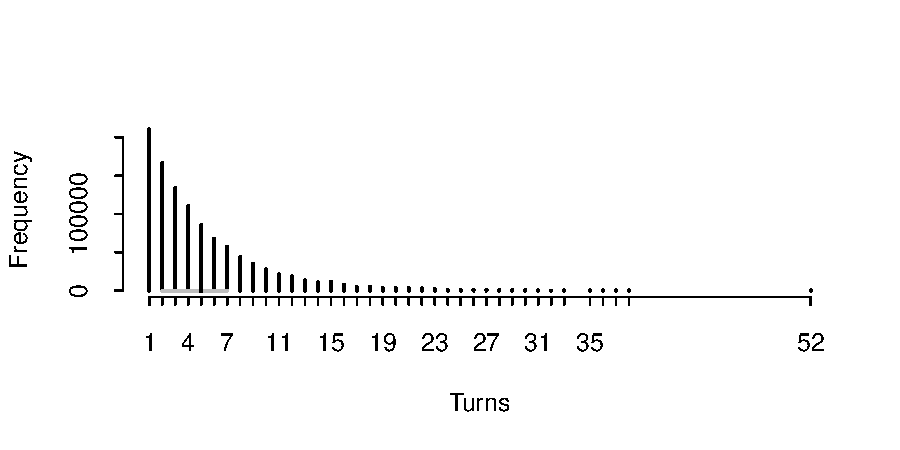
\includegraphics{door-find-frequency.pdf}%

The good news is that most of the time the player will find a door in
under 10 turns (about a 90\% chance). The bad news is if the RNG is in a
bad mood it may take significantly longer to find the door. If instead
the odds increase on repeated searches (that is, if the player searches
without moving\textendash moving resets the repeated search counter) via
something like the following:

\begin{verbatim}
int new_search(void)
{
    int turns = 0;
    while (1) {
        if (rnd(100) < 10 + 4 * turns++)
            break;
    }
    return turns;
}
\end{verbatim}

The initial odds are lower, though a simulation of this new
function shows that the long tail has been reduced to at most
\symbol{126}16 turns:

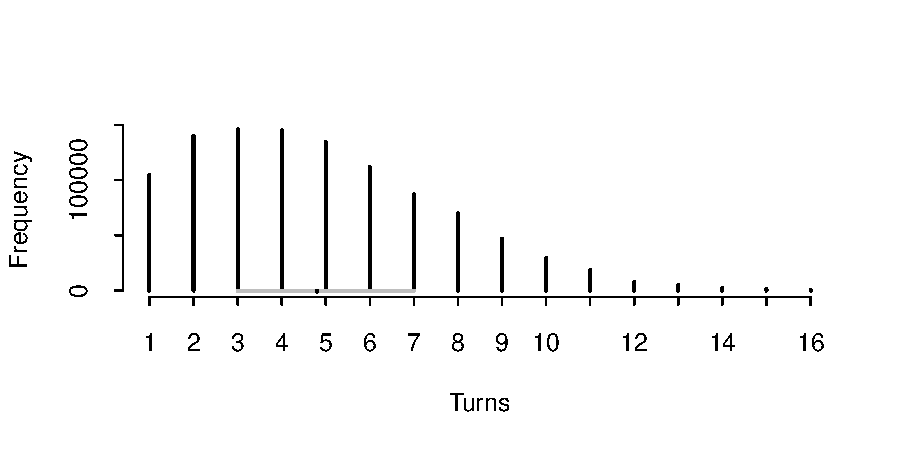
\includegraphics{new-door-find-frequency.pdf}%

\section*{Appendix Z}

ZAngband 2.6.2 presents portability problems, in particular 100\% CPU
use during character generation. This turns out to be a RNG problem.
Investigation of the source reveals that the RNG is
seeded\footnote{\url{https://flak.tedunangst.com/post/random-in-the-wild}}
poorly, much like the choice of a cup in an Indiana Jones movie.

\begin{verbatim}
% grep 'seed =' src/dungeon.c 
                seed = (time(NULL));
                seed = ((seed >> 3) * (getpid() * 2));
\end{verbatim}

However this is not cause of the CPU bug, rather a weakness that may be
exploited by a crafty player to guess or know what the RNG will roll,
one that may be fixed via \texttt{arc4random(3)} or by reading 32 bits
from \texttt{/dev/urandom}. \\

The CPU usage can be debugged up a macro, or rather a series of macros
in \texttt{src/z-rand.h} that have the bonus of not allowing my debugger
step through the critical \texttt{Rand\_div} function.

\begin{verbatim}
#define randint1(M) \
        (randint0(M) + 1)
#define randint0(M) \
        ((s32b)Rand_div(M))
\end{verbatim}

\texttt{Rand\_div} is complicated; it contains not one but two different
RNG. Replacing this entire function with an equivalent
\texttt{arc4random\_uniform} call leads to map generation failures due to
\texttt{arc4random\_uniform} being too random compared to what the
original function produces, in particular to the outputs of the "simple
RNG". So no simple fix here; the code depends on particular values from
the particular RNG used. The CPU bug, however, is in the "complex RNG"
portion of the code; somewhere in \texttt{src/birth.c} character
attributes are rolled up in the Dungeons \& Dragons tradition:

\begin{verbatim}
        while (TRUE)
        {
                /* Roll some dice */
                for (j = i = 0; i < 18; i++)
                {
                        /* Roll the dice */
                        dice[i] = randint1(3 + i % 3);
\end{verbatim}

with lots of dice rolls to obtain better stats; in a real-life game a
nice Dungeon Master would let a player re-roll a bad attribute roll;
here that instead is brute forced. (If you're going to allow the player
to obtain good stats, there are more CPU efficient ways to do that.
Anyways!) With lots of rolls, much time is spent in \texttt{Rand\_div} by
way of the \texttt{randint1} macro, which for debugging can be
temporarily replaced by a direct function call:

\begin{verbatim}
                        dice[i] = 1 + Rand_div(3 + i % 3);
\end{verbatim}

This in a debugger shows much spinning around in the loop:

\begin{verbatim}
                while (1) {
                        int j;
                        j = Rand_place + 1;
                        if (j == RAND_DEG) j = 0;
                        r = (Rand_state[j] += Rand_state[Rand_place]);
                        r = (r >> 4) / n;
                        Rand_place = j;
                        if (r < m) break;
                }
\end{verbatim}

Most values for \texttt{r} are larger than \texttt{m} so the loop almost
never exits, unless one is extremely patient or has an extremely fast
CPU. \texttt{m} is the input to \texttt{Rand\_div}, here values in the
range of three to five, inclusive. \texttt{r} meanwhile is \texttt{u32b}
which appears to be a unsigned 32-bit value, or what \texttt{stdint.h}
(now, but not when ZAngband was being developed) provides as
\texttt{uint32\_t}. Over in \texttt{src/h-type.h} we find:

\begin{verbatim}
/* Signed/Unsigned 32 bit value */
#ifdef L64      /* 64 bit longs */
typedef signed int s32b;
typedef unsigned int u32b;
#else
typedef signed long s32b;
typedef unsigned long u32b;
#endif
\end{verbatim}

Where \texttt{L64} is only set on DEC Alpha OSF systems. So on my 64-bit
system (OpenBSD 6.5, amd64) the \texttt{s32b} and \texttt{u32b} are
actually eight instead of four byte containers.

\begin{verbatim}
% cfu 'printf("%lu\n", sizeof(unsigned long))'
8
% cfu 'printf("%lu\n", sizeof(uint32_t))'     
4
\end{verbatim}

This well explains why the RNG has problems; the \texttt{Rand\_state} is
permuting 64-bit values instead of the expected 32-bit values\ldots
someone could work out exactly why this is bad for the algorithm
involved, but the fix here is to make \texttt{s32b} and \texttt{u32b}
use proper 32-bit containers on all 64-bit systems.

\end{document}
